\documentclass[../DoAn.tex]{subfiles}
\usepackage{booktabs}
\begin{document}

\section{Ngữ cảnh của bài toán}
Hiện nay, với sự phát triển mạnh mẽ của lĩnh vực y sinh khiến cho chí phí cho công việc giải trình tự gene giảm đi đáng kể. Việc naỳ cũng kéo theo số lượng các báo cáo khoa học về giải trình tự gene tăng theo cấp số nhân. Những mô tả biến thể và gene được đề cập trong bài báo này có thể được sử dụng lại bởi các đơn vị giải trình tự gene. Vì thế, việc thu thập, tìm kiếm các thông tin này một cách nhanh chóng, tự động là nhu cầu thực tế. Mặc dù, chất lượng tốt nhất vẫn là tìm kiếm và xác thực thủ công bởi các chuyên gia. Tuy nhiên, việc tìm kiếm và tổng hợp tự động cũng rất có ích vì nó có thể đẩy nhanh tốc độ và làm giảm đáng kể công sức xác thực thủ công. Bên cạnh sự phát triển của lĩnh vực y sinh, khoa học máy tính cũng có những bước tiến rất đáng kể trong việc phát triển những thuật toán xử lý ngôn ngữ tự nhiên với độ chính xác cao, tốc độ nhanh. Chính vì thế, trong đồ án tốt nghiệp này, em đề xuất một phương pháp áp dụng các thuật toán học máy, để giải quyết bài toán thu thập dữ liệu bài báo liên quan đến ung thư và xác định các đột biến gene tương ứng.

\section{Các kết quả nghiên cứu tương tự}
\subsection{Using Machine Learning and Natural Language Processing to Review and Classify the Medical Literature on Cancer Susceptibility Genes}
Trong bài báo này, các tác giả đã xây dựng mô hình phân loại văn bản, với mục đích phân loại các bài báo khoa học đề cập đến các gene nhạy cảm với ung thư. Bộ dữ liệu được sử dụng bao gồm tiêu đề và tóm tắt của 3,919 bài báo được gán nhãn thủ công. Các bài báo này được thu thập từ cơ sở dữ liệu Pubmed. Để giải quyết vấn đề này, các tác giả đã đề xuất 2 mô hình phân loại văn bản là SVM và CNN. 
Mô hình đầu tiên là SVM với với phương pháp trích chọn đặc trưng là bag of ngrams. Mô hình thứ hai là CNN, mô hình này mô hình nhận trực tiếp đầu vào là tiêu đề và tóm tắt đã được tokenize. Cả 2 mô hình được đánh giá qua hai nhiệm vụ phân loại độ thấm của gene (Penetrance) và mức độ phổ biến của gene (Prevalence). 

% \usepackage{booktabs}
\begin{table}[]
\caption{Hiệu năng của 2 mô hình phân loại văn bản}
\label{tab:svmcnn}
\begin{tabular}{@{}|l|cc|cc|@{}}
\toprule
        & \multicolumn{2}{c|}{độ thấm của gene (Penetrance)} & \multicolumn{2}{c|}{độ phổ biến của gene (Prevalence)} \\ \midrule
Mô hình & \multicolumn{1}{c|}{Độ chính xác}    & F1 score    & \multicolumn{1}{c|}{Độ chính xác}      & F1 score      \\ \midrule
SVM & \multicolumn{1}{c|}{0.8893} & 0.7753 & \multicolumn{1}{c|}{0.8892} & 0.8329 \\ \midrule
CNN & \multicolumn{1}{c|}{0.8853} & 0.7523 & \multicolumn{1}{c|}{0.8852} & 0.8210 \\ \bottomrule
\end{tabular}
\end{table}

Bảng \ref{tab:svmcnn} Hiệu năng của hai mô hình phân loại văn bản SVM và CNN được đề xuất trong bài báo \cite{useML}.
Với kết quả này, có thể thấy rằng, cách tiếp cận phân loại văn bản y khoa theo hướng xử lý ngôn ngữ tự nhiên có thể cho kết quả tốt. Tuy nhiên, cách tiếp cận này cũng có hạn chế nhất định. Mô hình tác giả đề xuất hoạt động không tốt đối với bài báo khoa học không có tóm tắt, hoặc có tóm tắt không đầy đủ.

\subsection{GAPscreener: An automatic tool for screening human genetic association literature in PubMed using the support vector machine technique \cite{GAPscreener}}
Với mong muốn xây dựng một công cụ sàng lọc dữ liệu là các bài báo đề cập đến gene người trên cơ sở dữ liệu pubmed, nhóm tác giả đã đề xuất sử dụng thuật toán phân loại support machine learning để xây dụng một công cụ phân loại văn bản. Để chuẩn bị dữ liệu training, họ đã thu thập ngẫu nhiên 10.000 tóm tắt của bài báo khoa học được xuất bản từ năm 2001 đến 2006 trên PubMed làm tập dữ liệu nền. Bộ dữ liệu dương tính (positive) gồm 10.000 bài báo liên quan đến gene bệnh được chọn
ngẫu nhiên từ cơ sở dữ liệu HuGE Navigator\cite{huge}, một cơ sở dữ liệu được cập nhật liên tục về các nghiên cứu liên quan đến dịch tễ học bộ gen người. Sau quá trình tiền xử lý dữ liệu, và huấn luyện mô hình, nhóm tác giả đã sử dụng toán SVM với hạt nhân là RBF để đạt hiệu quả phân loại tốt nhất. Qua đó chỉ số recall của mô hình khá tốt đạt 0.975. VỚi kết quả này, nhóm tác giả đã có thể xây dựng được một công cụ sàng lọc văn bản y khoa với hiệu suất rất cao, chỉ với một số lượng không lớn dữ liệu (20.000 văn bản). Tuy nhiên , thời gian chạy của thuật toán là 0.02s mỗi tóm tắt là chưa thực sự ấn tượng.

\section{Tổng quan về học máy}
\label{section:3.1}
\subsection{Học máy là gì}
Trí tuệ nhân tạo là một nhánh của khoa học máy tính, là một nhóm các thuật toán giúp cho máy tính có thể bắt chước hành vi của con người như khả năng hiểu (understanding), khả năng học tập (studying), khả năng suy luận (inference), khả năng ra quyết định (decision making). 

Học máy (Machine Learning) là một tập con của Trí tuệ nhân tạo, giúp máy tính có khả năng học từ dữ liệu cho trước mà không cần các luật quyết định cho sẵn. Hiện nay ứng dụng của học máy hay trí tuệ nhân tạo đã có mặt ở rất nhiều lĩnh vực của đời sống xã hội như hệ thống lọc thư điện tử rác (spam), tính năng nhận diện khuôn mặt trên iphone, hệ thống gợi ý trên ứng dụng stream nhạc spotify, hệ thống xe tự lái của Tesla, Waymo, ...
\subsection{Phân loại các thuật toán học máy}
Có nhiều cách để phân loại các thuật toán học máy, thông thường, ta có thể phân loại theo 2 cách:
\textbf{Phân loại dựa trên phương thức học}
\begin{enumerate}
    \item Học có giám sát
    \item Học không giám sát
    \item Học bán giám sát
    \item Học tăng cường
\end{enumerate}

\textbf{Phân loại dựa trên chức năng}
\begin{enumerate}
    \item Phân loại
    \item Hồi quy
    \item Chính quy
    \item Phân cụm
    \item Giảm chiều dữ liệu
    \item Mạng nơ ron nhân tạo
\end{enumerate}

\subsection{Trích chọn đặc trưng - Feature engineering}
Về mặt toán học , các thuật toán học máy sẽ cố gắng xử lý một điểm dữ liệu có dạng là một vector nhiều chiều, trong đó mỗi phần tử thuộc vector là một đặc trưng. Tuy nhiên, trong thực tế, dữ liệu đều không tồn tại ở dạng vector. Đối với bộ dữ liệu ImageNet \cite{deng2009imagenet} hay COCO \cite{lin2014microsoft} , mỗi điểm dữ liệu là một bức ảnh, ta có thể coi mỗi bức ảnh là một tensor 3d. Hay đối với bài toán về xử lý ngôn ngữ tự nhiên, dữ liệu cũng tồn tại ở dạng văn bản. Trong bài toán xử lý giọng nói, dữ liệu tồn tại ở dạng tín hiệu. Trong bài toán về dự đoán hình dạng 3d của phân tử protein, dữ liệu tồn tại ở dạng đồ thị (graph)... Chính vì thế, trước khi làm việc với các thuật toán học máy, đầu tiên ta cần chuyển đổi dữ liệu thô ban đầu sang dạng vector. Việc biến đổi từ dữ liệu thực sang dạng vector được gọi là "trích xuất đặc trưng". Vector này được sử dụng làm đại diện cho dữ liệu thực ban đầu trong bài toán học máy. 

Trong cùng một bài toán, các vector đặc trưng đều yêu cầu có kích thước là như nhau. Khi đó, toàn bộ dữ liệu có thể được lưu trữ ở dạng matrận, trong đó, mỗi hàng hoặc mỗi cột là vector feature của một điểm dữ liệu. Ngoài ra, kích thước các vector đặc trưng giống nhau cũng là điều kiện để thực hiện các phép tính trên những vector đó như tích vô hướng, tích có hướng, cộng hai vector, trừ hai vector, ... 

Đối với bài toán thị giác máy tính (Computer Vision), với đầu vào là một bức ảnh, ta có thể coi mỗi pixel của bức ảnh là một đặc trưng, tập hợp tất cả những pixel chính là một vector đặc trưng đại diện cho bức ảnh đó. Ngoài ra ta có thể sử dụng các phương pháp khác như Histogram of Oriented Gradients (HOG) \cite{1467360}, Scale-Invariant Feature Transform (SIFT) \cite{sift}, hay sử dụng phép tính tích chập (Convolutional)...

Đối với bài toán xử lý ngôn ngữ tự nhiên (natural language processing–NLP), phương pháp đang được sử dụng phổ biến được gọi là "túi đựng từ" (Bag-of-words). Phương pháp này xây dựng một từ điển bao gồm tất cả các từ xuất hiện trong bộ dữ liệu. Với mỗi văn bản, ta tạo một vector đặc trưng có kích thước bằng kích thước của từ điển. Mỗi phần tử của vector đại diện cho 1 từ trong từ điển. Giá trị của một phần tử trên vector thể hiện số lần xuất hiện của từ đó trong văn bản.

\subsection{Một số thuật học máy điển hình}
\subsubsection{Hồi quy logistic - Logistic regression}
Các thuật toán phân loại trong học máy đều cố gắng đưa ra một đường (mặt) phân chia giữa 2 (nhiều) nhóm dữ liệu. Trong thực tế, hầu hết dữ liệu đều tồn tại ở dạng non linear separable data (không tồn tại một đường thẳng, siêu phẳng phân tách giữa 2 nhóm dữ liệu). Chính vì thế, thuật toán hồi quy tuyến tính (linear regression) sẽ không thể giải quyết được vấn đề này. Để có thể làm được điều này, hồi quy logistic sử dụng hàm sigmoid.  \[\sigma (x)= \frac{1}{1+e^{-x}}\]Thêm vào đó, hàm sigmoid nhận giá trị trong khoảng [0,1], do đó, ta có thể coi đầu ra của hàm sigmoid là xác suất đại diện cho lớp cần phân loại.
\begin{figure}
    \centering
    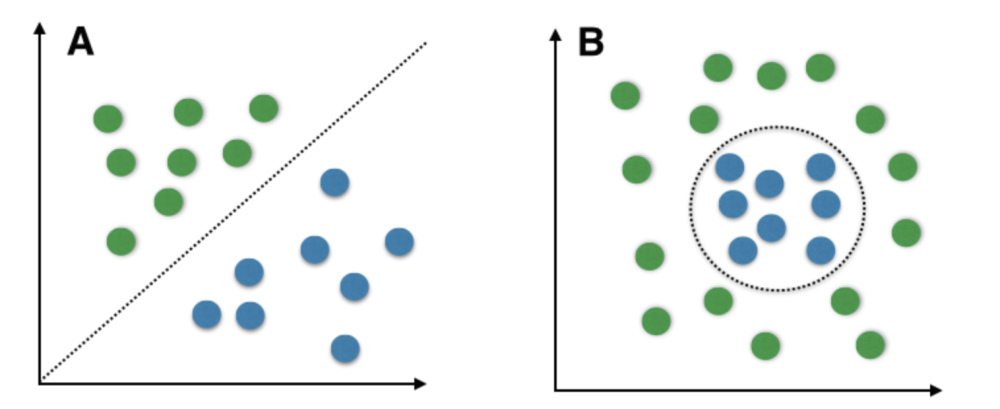
\includegraphics[width=1\linewidth]{Hinh_ve/linear_sep.png}
    \caption{Hình A: Dữ liệu tồn tại đường thẳng (linear) phân chia giữa 2 lớp (class) Hình B: không tồn tại đường thẳng phân chia giữa 2 loại dữ liệu}
    \label{fig:hình1}
\end{figure}

\begin{figure}
    \centering
    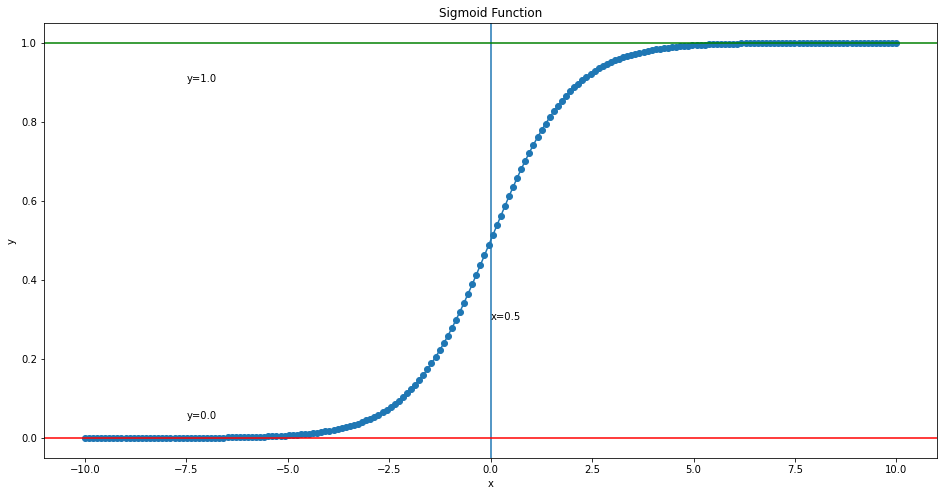
\includegraphics[width=1\linewidth]{Hinh_ve/sigmoid_function.png}
    \caption{Đồ thị hàm sigmoid, hàm sigmoid có giá trị nằm trong đoạn [0, 1]}
    \label{fig:hình2}
\end{figure}

\subsubsection{Máy vector hỗ trợ - support vector machine- SVM}
SVM là một thuật toán học có giám sát, SVM nhận dữ liệu đầu vào và phân loại chúng thành 2 lớp khác nhau. SVM sẽ xây dựng một siêu phẳng (khái niệm mặt phẳng trong không gian lớn hơn 3 chiều) phân chia 2 lớp dữ liệu với nhau. Khoảng cách từ siêu phẳng tới 2 lớp dữ liệu là lớn nhất có thể, và sự chênh lệch giữa khoảng cách từ siêu phẳng đến 2 lớp dữ liệu là nhỏ nhất có thể.

Tuy nhiên, đối với dữ liệu non linear separable, ta không thể tìm được siêu phẳng phân chia 2 lớp dữ liệu. Để giải quyết vấn đề này, thay vì đi tìm đường phân chia dạng phi tuyến như thuật toán hồi quy logistic, SVM sẽ sử dụng một phương pháp được gọi là kernel SVM. kernel SVM bản chất là một hàm số , biến đổi điểm dữ liệu từ không gian vector cũ sang không gian vector mới có nhiều chiều hơn, và việc phân tách dữ liệu trong không gian mới là dễ dàng hơn so với không gian vector cũ. Một số hàm kernel thông dụng có thể kể đến như:
\begin{enumerate}
    \item Tuyến tính (Linear)
    \item Đa thức (Polynomial)
    \item Radial Basic Function
    \item Sigmoid
\end{enumerate}
Ngoài ra, tùy thuộc vào từng loại dữ liệu ta cũng có thể tự định nghĩa các hàm kernel.
Các kernel SVM có độ phức tạp tính toán O(n2) cho quá trình training và O(nd) cho quá trình phân loại (n là số lượng điểm dữ liệu đầu vào, d là số chiều của điểm dữ liệu). Thay vào đó, kernel tuyến tính chỉ có độ phức tạp O(nd) cho training và O(d) cho quá trình phân loại. Chính vì thế, đối với dữ liệu có số lượng chiều của dữ liệu lớn (ví dụ như bài toán về xử lý ngôn ngữ tự nhiên), ngoài việc quan tâm đến độ chính xác của thuật toán, ta cũng cần quan tâm đến chi phí tính toán. 

\subsubsection{Naive Bayes classifier}
Naive Bayes là một thuật toán phân loại nhiều lớp hoạt động với 2 giả thiết: giả thiết thứ nhất là dữ liệu (data) và lớp (class) là 2 biến ngẫu nhiên độc lập với nhau. Giả thiết thứ 2 là các đặc trưng của vector đặc trưng cũng là các biến ngẫu nhiên độc lập với nhau. Có thể thấy rằng trong thực tế, rất khó để tìm được bộ dữ liệu nào thỏa mãn 2 điều kiện về độc lập tuyến tính như trên, và việc khẳng định được 2 biến ngãu nhiên là độc lập với nhau cũng là một bài toán phức tạp. Tuy nhiên, những giả thiết ngây ngô này lại giúp cho thuật toán hoạt động rất hiệu quả cả về đô chính xác lẫn chi phí tính toán. Chính vì chi phí tính toán thấp ngay cả khi kích thước của vector đặc trưng là lớn, thuật toán này rất phù hợp để giải quyết các bài toán phân loại văn bản.

\subsubsection{K láng giềng gần nhất - K-nearest neighbor - kNN}
kNN là một thuật toán được sử dụng cho cả hai nhiệm vụ là hồi quy và phân loại. kNN cũng là mô hình không có tham số  và không cần quá trình training. Mọi tính toán của thuật toán sẽ diễn ra khi cần tính toán kết quả của dữ liệu mới. kNN sẽ đi tìm đầu ra của một điểm dữ liệu mới bằng cách chỉ dựa trên thông tin của K điểm dữ liệu trong dữ liệu gần nó nhất (K-lân cận), kNN không quan tâm đến việc có một vài điểm dữ liệu trong những điểm gần nhất này là nhiễu hay không. Nếu điểm dữ liệu mới gần với điểm dữ liệu của lớp (class) nào hơn thì kNN sẽ phân chia điểm dữ liệu mới này vào lớp dữ liệu đó.

\begin{figure}
    \centering
    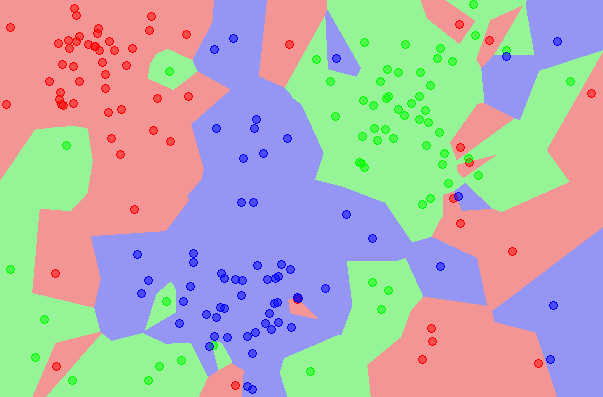
\includegraphics[width=1\linewidth]{Hinh_ve/Map1NN.png}
    \caption{Bản đồ của kNN với k = 1(Nguồn: \href{https://en.wikipedia.org/wiki/K-nearest_neighbors_algorithm}{wikipedia})}
    \label{fig:hình3}
\end{figure}

\subsection{Đánh giá hệ thống phân lớp}
Đối với các thuật toán học máy, không có công thức chung cho việc xác định thuật toán nào là phù hợp với dữ liệu này mà không phù hợp với dữ liệu khác. Vì thế ta phải tiến hành đánh giá chúng. Đối với các thuật toán phân loại cũng như vậy. Hiệu quả của mô hình được đánh giá trên dữ liệu kiểm tra (data test) . Ta sẽ sử dụng mô hình để dự đoán xem dữ liệu test thuộc về lớp (class) nào. Kết quả dự đoán thu được sẽ so sánh với nhãn (label) của dữ liệu đó. Có nhiều cách để đánh giá độ hiệu quả của mô hình phân lớp. Tùy thuộc vào bài toán và kỳ vọng của ta với bài toán đó mà ta sẽ lựa chọn phéo đánh giá phù hợp.
\subsubsection {Độ chính xác - Accuracy}
Phương pháp đơn giản và hay được sử dụng nhất là độ chính xác. Phương pháp này đơn giản là tính tỉ lệ giữa số điểm dữ liệu mô hình dự đoán đúng chia cho tổng số điểm dữ liệu. Phương pháp này khá đơn giản, tuy nhiên chỉ số này không đáng tin cậy khi dữ liệu kiểm tra bị mất cân bằng (unbalance data). Ngoài ra, "độ chính xác" không thể hiện được độ chính xác trên từng lớp dữ liệu (class).
\subsubsection {Ma trận nhầm lẫn - Confusion matrix}
"Ma trận nhầm lẫn" có ưu điểm hơn so với "độ chính xác" là thể hiện được rõ ràng có bao nhiêu điểm dữ liệu được mô hình dự đoán đúng, có bao nhiêu điểm dữ liệu bị dự đoán sai, trong trường hợp bị dự đoán sai thì những điểm dữ liệu đó bị mô hình phân chia vào lớp dữ liệu (class) nào. 

\begin{figure}
    \centering
    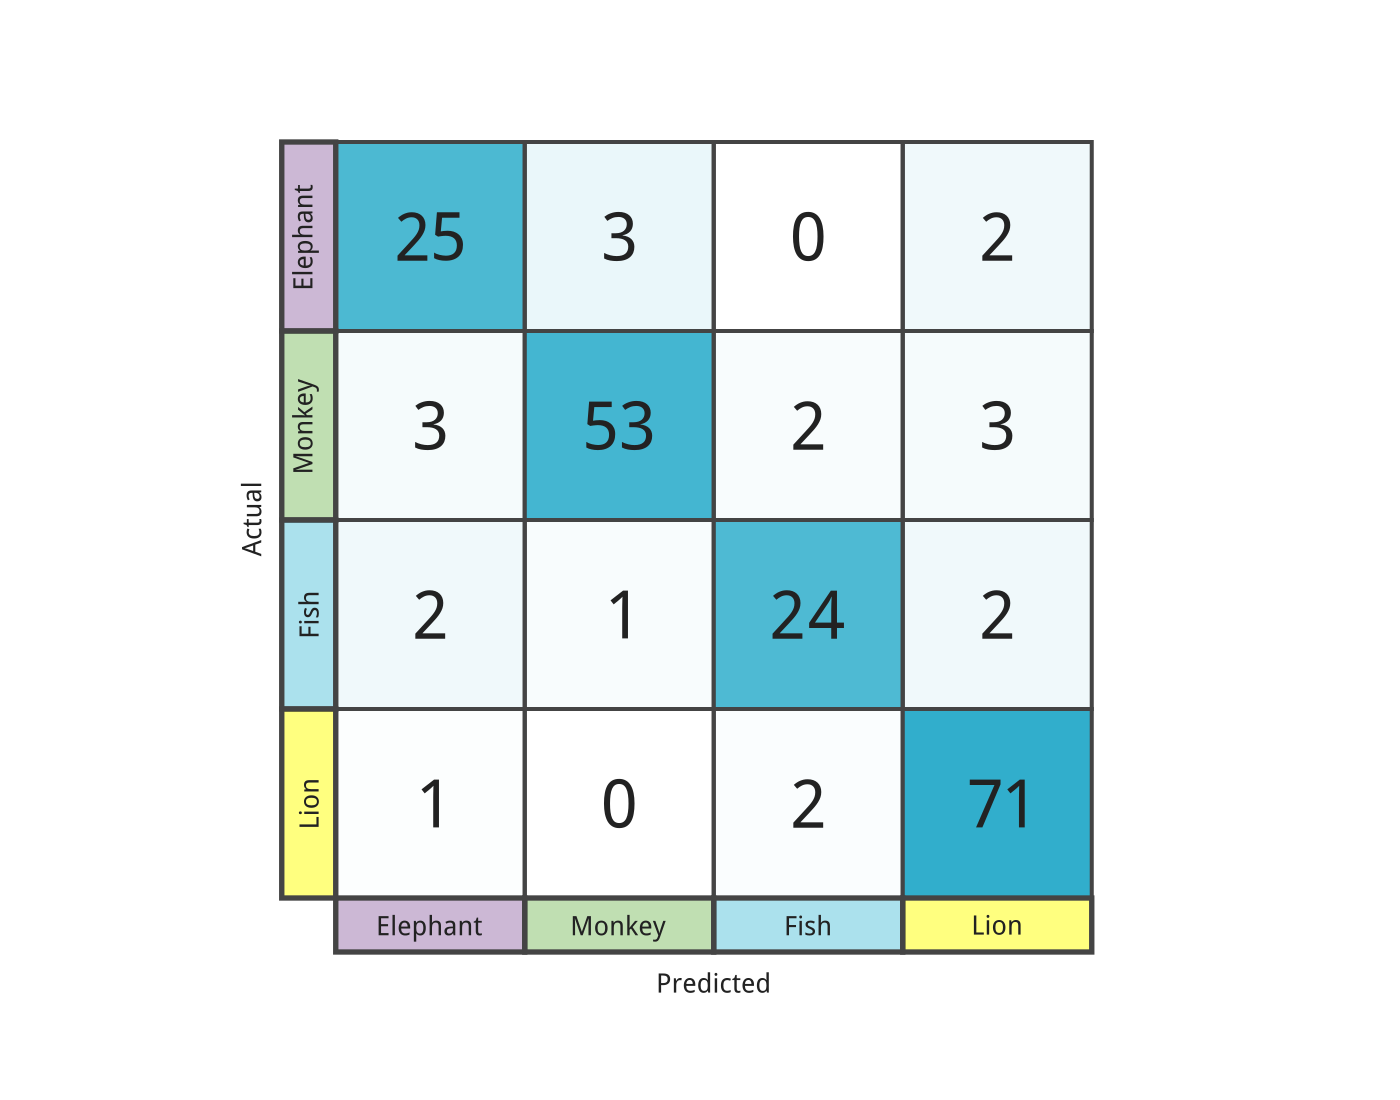
\includegraphics[width=1\linewidth]{Hinh_ve/Confuse_matrix.png}
    \caption{Ma trận nhầm lẫn cho bài toán phân loại 4 lớp dữ liệu. Đối với lớp dữ liệu "Elephant" , dữ liệu kiểm tra có 30 điểm dữ liệu , mô hình dự đoán đúng 25 điểm dữ liệu, mô hình dự đoán sai 5 điểm dữ liệu trong đó có 3 điểm dữ liệu mô hình dự đoán vào lớp dữ liệu "Monkey", 2 điểm dữ liệu mô hình dự đoán vào lớp dữ liệu "Lion" (Nguồn: \href{https://towardsdatascience.com/visual-guide-to-the-confusion-matrix-bb63730c8eba}{Towards Data Science})}
    \label{fig:hinh4}
\end{figure}

\subsubsection{Precision và Recall}
Khi bộ dữ liệu bị mất cân bằng rất nhiều (unbalance data) , khi đó, "độ chính xác" không thể hiện phản ánh chính xác khả năng phân loại của mô hình. Khi đó, ta sử dụng một chỉ số khác là "độ chuẩn xác"(Precision) và "thu hồi" (Recall). Giống như "Độ chính xác", hai chỉ số này cũng nhận giá trị trong đoạn [0, 1].  

\begin{figure}
    \centering
    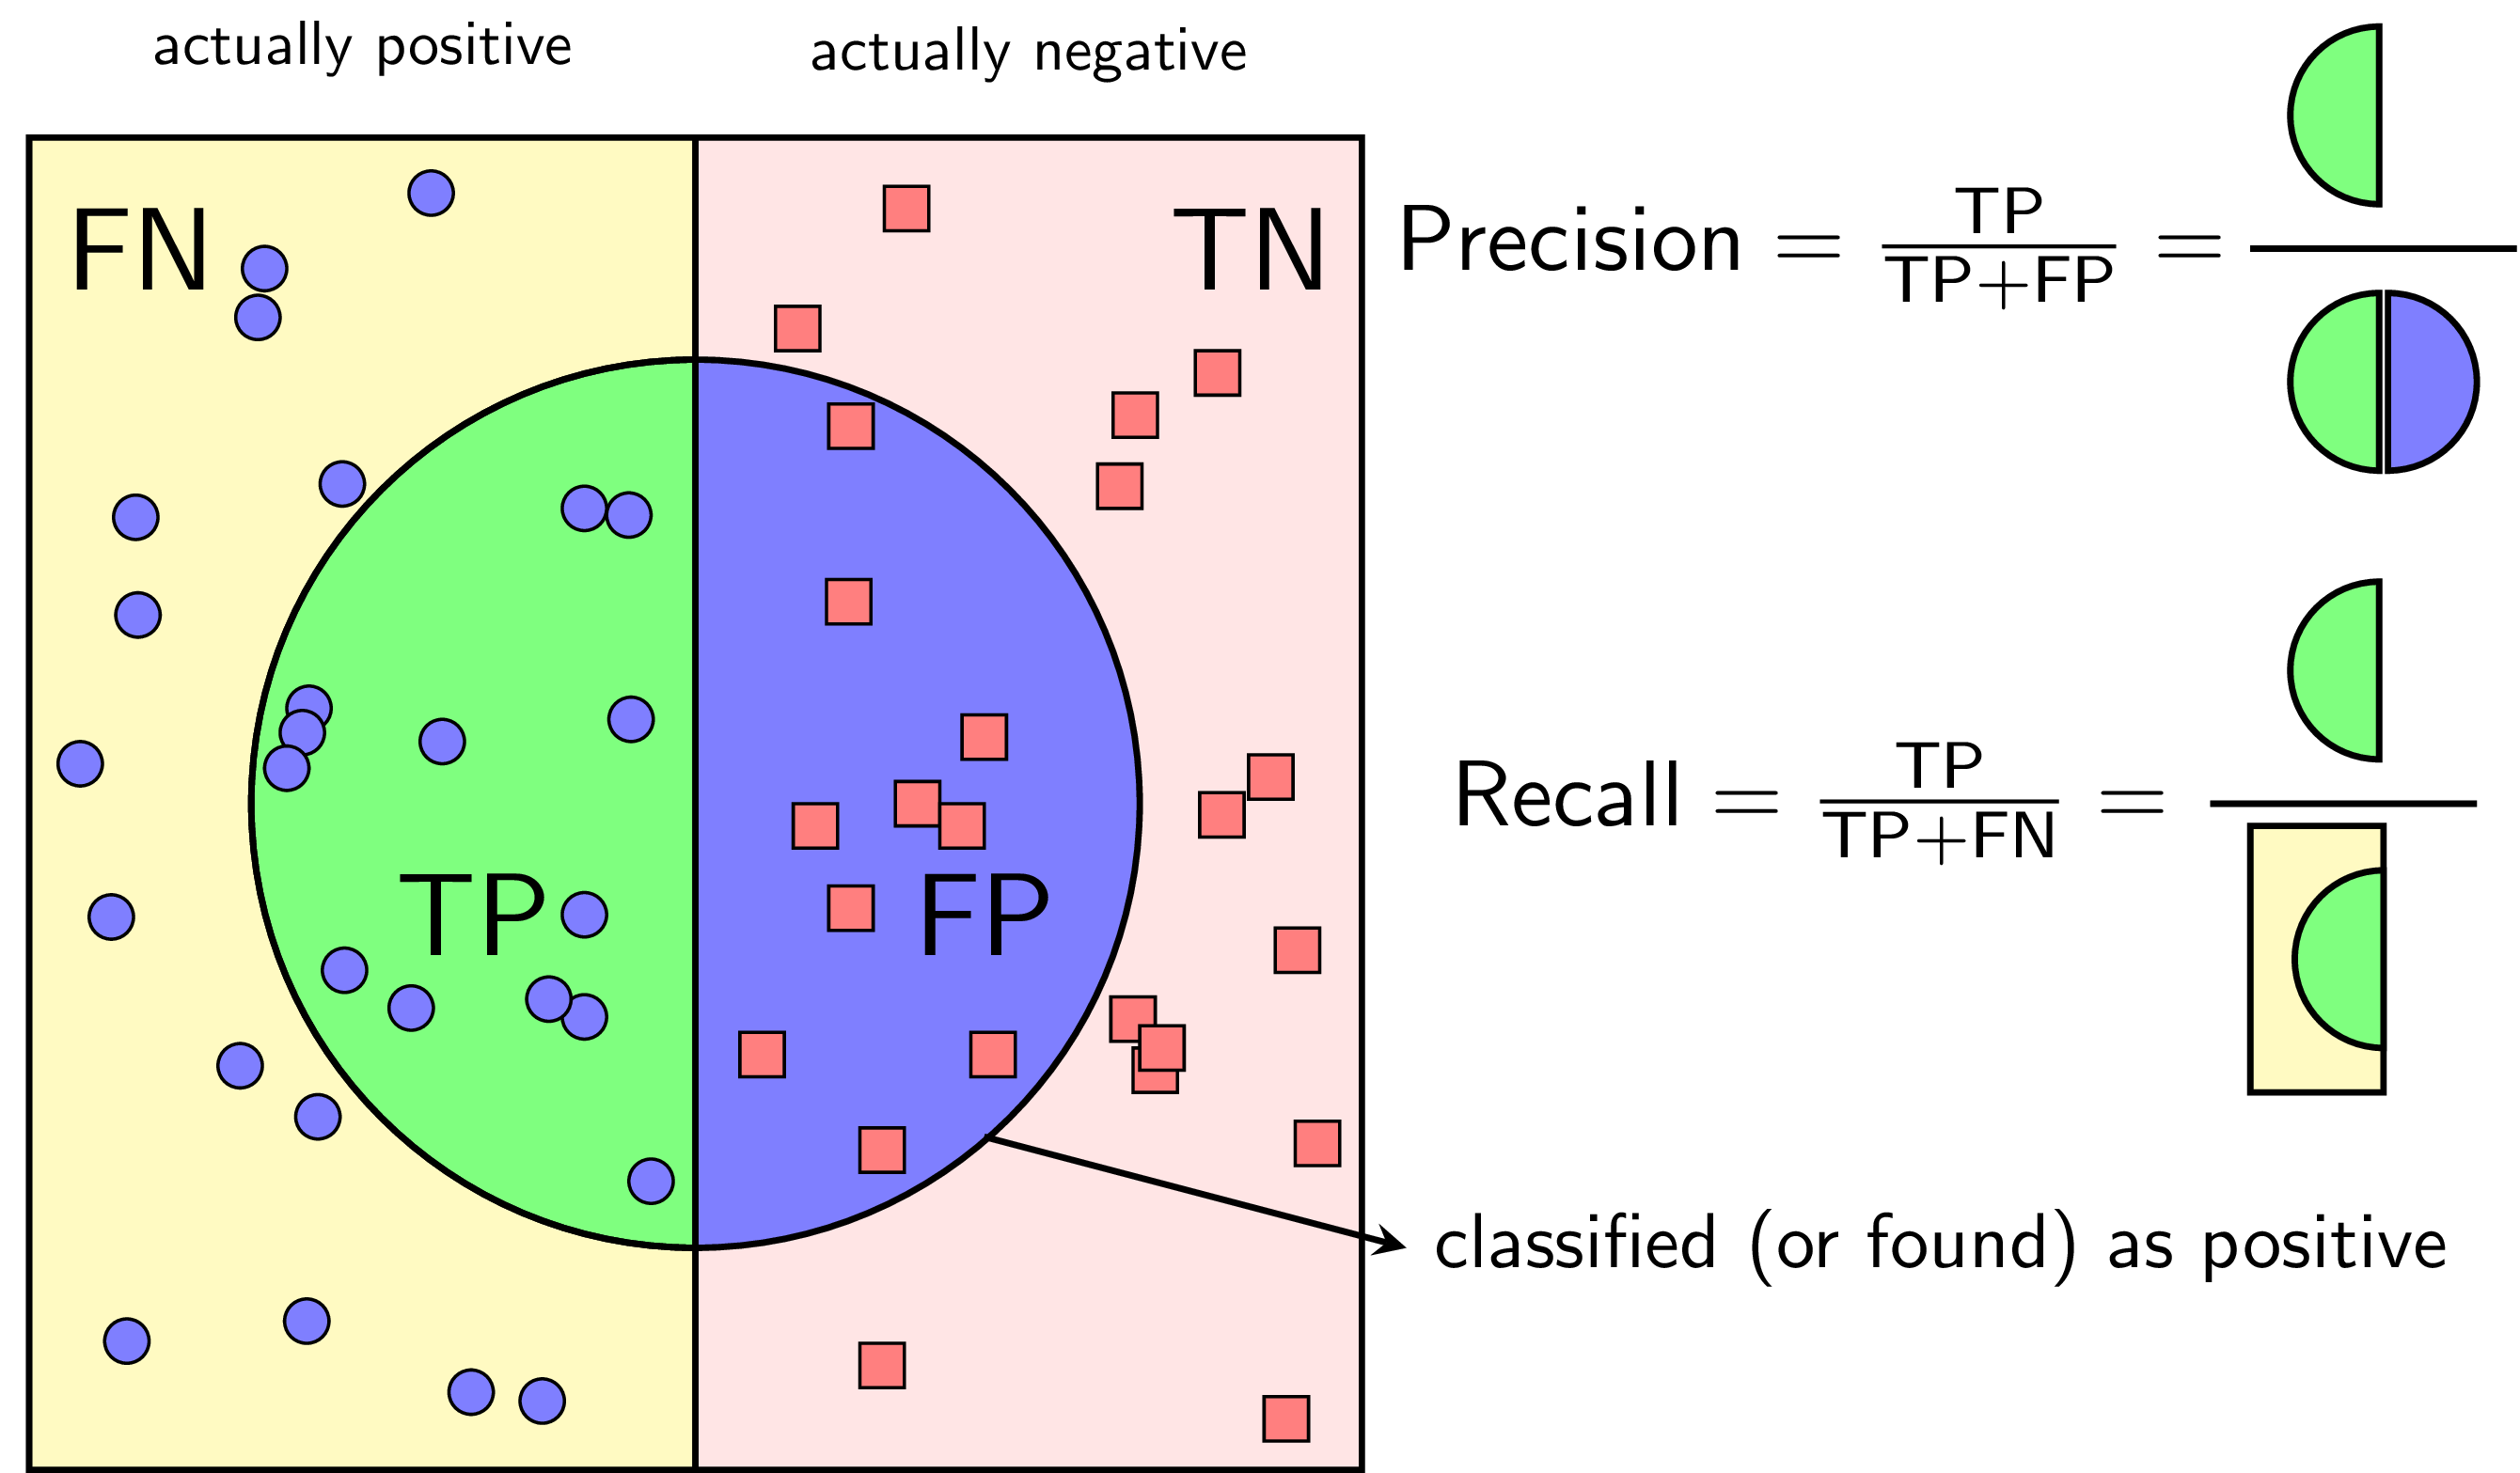
\includegraphics[scale=.15]{Hinh_ve/Precision_Recall.png}
    \caption{Cách tính Precision và Recall. Nguồn: https://machinelearningcoban.com}
    \label{fig:hinh5}
\end{figure}

Chỉ số "Precision" càng cao có nghĩa là trong những điểm positive được tìm thấy, có rất ít điểm dữ liệu negative. Chỉ số "Recall" cao có nghĩa là trong toàn bộ dữ liệu kiểm tra, tỉ lệ điểm dữ liệu positive được phân loại là positive là rất cao. Trong các bài toán phân loại, ta đều mong muốn 2 chỉ số này càng cao càng tốt. Một mô hình phân loại tốt sẽ có chỉ số Precision và Recall cao, nhưng ngược lại, chỉ số Precision hoặc Recall cao không đồng nghĩa với việc mô hình phân loại hoạt động tốt. 

\end{document}